\section*{Arquitetura, Execução e Debug da CPU}
\setcounter{exercicio}{0}

\gabaritoex{1}
Para atender aos requisitos propostos, a arquitetura original da CPU do Z01.1
deve ser estendida conforme descrito a seguir:

Um novo registrador \texttt{\%S} deve ser inserido no banco de registradores da CPU,
de forma análoga aos registradores existentes \texttt{\%A} e \texttt{\%D}.
Esse registrador deve possuir largura de 16 bits e estar conectado ao barramento
interno de dados.

A linguagem de máquina deve ser estendida para permitir que o registrador
\texttt{\%S} seja selecionado como origem ou destino em instruções do tipo C.
Isso implica a ampliação dos campos de seleção de registradores na instrução
(binários adicionais no campo de destino e/ou origem).

Para permitir a instrução \texttt{movw \%A, (\%D)}, o registrador \texttt{\%D}
deve ser conectado ao barramento de endereços da memória RAM, funcionando como
um registrador de endereçamento alternativo ao \texttt{\%A}.

Para permitir a instrução \texttt{leaw \$5, \%D}, a lógica de carregamento imediato
deve ser estendida de modo que o valor proveniente da ROM possa ser direcionado
não apenas ao registrador \texttt{\%A}, mas também ao registrador \texttt{\%D}.
\begin{center}
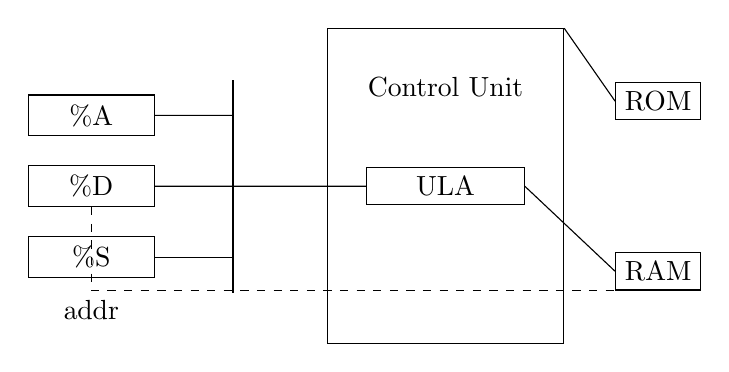
\begin{tikzpicture}[scale=0.9]

% Registradores
\node[draw, minimum width=1.6cm] (A) at (0,2) {\%A};
\node[draw, minimum width=1.6cm] (D) at (0,1) {\%D};
\node[draw, minimum width=1.6cm] (S) at (0,0) {\%S};

% Barramento
\draw[thick] (2,-0.5) -- (2,2.5);

% CPU
\node[draw, minimum width=3cm, minimum height=4cm] (CPU) at (5,1) {};
\node at (5,2.4) {Control Unit};
\node[draw, minimum width=2cm] (ALU) at (5,1) {ULA};

% Memórias
\node[draw] (ROM) at (8,2.2) {ROM};
\node[draw] (RAM) at (8,-0.2) {RAM};

% Conexões
\draw (A.east) -- (2,2);
\draw (D.east) -- (2,1);
\draw (S.east) -- (2,0);

\draw (2,1) -- (ALU.west);
\draw (ALU.east) -- (RAM.west);
\draw (CPU.north east) -- (ROM.west);

% Endereçamento via D
\draw[dashed] (D.south) |- node[below]{addr} (RAM.south);

\end{tikzpicture}
\end{center}


\textit{A linha tracejada indica o novo caminho de endereçamento da RAM via o registrador \%D.}


\gabaritoex{2}
A instrução \texttt{nop} não altera o estado do sistema, apenas avança o PC.

\gabaritoex{3}
A CPU não executa simultaneamente essas instruções devido à arquitetura
sequencial.

\gabaritoex{4}
O sinal \texttt{loadPC} controla o avanço ou salto do contador de programa.

\gabaritoex{5}
A falha ocorre devido à ativação incorreta do sinal de carregamento do
registrador \%A durante a execução da instrução \texttt{addw \%A, \%D, (\%A)}.
O registrador \%A deveria apenas fornecer o endereço de memória, mas acaba
sendo sobrescrito no mesmo ciclo, resultando em acesso inválido à RAM.


\gabaritoex{6}
Os comandos executados são:
\begin{verbatim}
leaw $1, %A
movw (%A), %D
addw %D, %A, %A
\end{verbatim}
\newpage